\documentclass{article}
\newcommand{\nm}{\begin{equation}}
\newcommand{\enm}{\end{equation}}
\newcommand{\nma}{\begin{align*}}
\newcommand{\enma}{\end{align*}}
\newcommand{\lp}{\left(}
\newcommand{\rp}{\right)}
\usepackage[utf8]{inputenc}
\usepackage{graphicx}
\usepackage{amssymb}
\usepackage{physics}
\title{statemech density operators}
\author{seth iwan }
\date{January 2020}

\begin{document}

\maketitle
\section{problem 1}
\textbf{what are the prbabilities of measureint $\ket{\pm}$ for these three staes}\\ 
\nm
\ket{\pm}=\ket{0}\pm\ket{1}
\enm
\\
\textbf{case 1:}\\
\\
\centerline{ 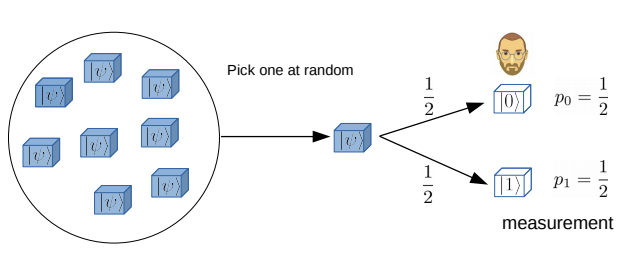
\includegraphics[scale=.5]{images-for-density-operator/case1.png}}\\
\textbf{solution:}\\
	\nm
	\rho = | \bra{\pm}\ket{\psi} |^2= |\lp\bra{0}\pm\bra{1}\rp *\frac{1}{\sqrt{2}} \lp\ket{0}+\ket{1}\rp|^2
	\enm
	
	\nm
	= \frac{1}{2} \pm \frac{1}{2}
	\enm
so the probability to measure $\ket{+}$ is 1 while the prbability to mesure $\ket{-}$ is zero

\textbf{case 2:}\\
\\
\centerline{ 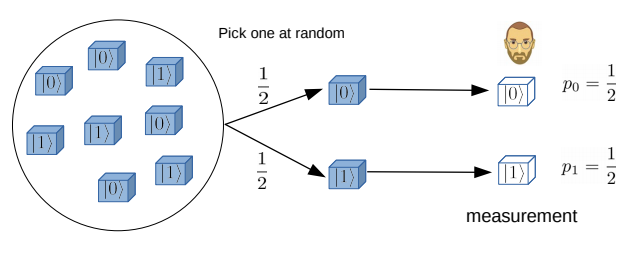
\includegraphics[scale=.5]{images-for-density-operator/case2.png}}\\
\textbf{solution:}\\
	since the state are either $\ket{0}$ or $\ket{1}$ there is 0 probability to be in $\ket{\pm}$ which is a sumation of those two states\\
\\

\textbf{case 3:}\\
\\
\centerline{ 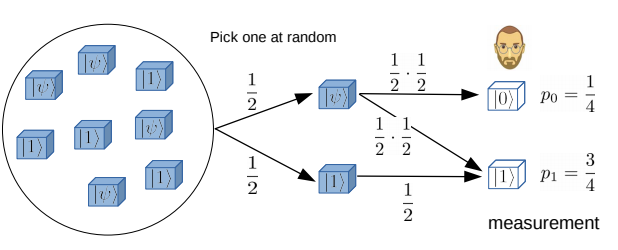
\includegraphics[scale=.5]{images-for-density-operator/case3.png}}\\
\textbf{solution:}\\

	
	\begin{align*}
	\rho_{\ket{+}}&=|\bra{+}\ket{\psi}|^2=1 \\
	\rho_{\ket{-}}&=|\bra{-}\ket{\psi}|^2=0 \\
	\end{align*}
but $\ket{\psi}$ has 1/2 chance of being measured, therfore $\ket{+}$ has 1/2 chance of being measured and $\ket{-}$ has zero chance of being measured.
\newpage
%%%%%%%%%%%%%%%%%%%%%%%%
%%%%%%%%%%%%%%%%%%%%%%%%

\textbf{question: a system is in a pure state $\ket{\Psi}=\frac{1}{\sqrt{2}}\ket{0}+\frac{1}{\sqrt{2}}\ket{1}$ . find teh density matrix in $\ket{0}$ and $\ket{1}$} \\
\textbf{solution:}
since it is a pure state the density opertaor isjust the outer product of $\ket{\Psi}$
\nm
\rho = \frac{1}{2}\lp \ket{0}\bra{0}+\ket{0}\bra{1}+\ket{1}\bra{0}+\ket{1}\bra{1}\rp
\enm
to get this in matrix formation in the basis $\ket{0}$ and $\ket{1}$ we do $\rho=\sum_i\sum_j\op{\psi_i}{\psi_i}\rho\op{\psi_j}{\psi_j}$ . so the density matrix is
\nm
\frac{1}{2}\mqty[1 & 1 \\ 1 & 1 ]
\enm


%%%%%%%%%%%%%%%%%%%%%%%
%%%%%%%%%%%%%%%%%%%%%%%
\section{problem: show that the purity is less than one, that is tr$\rho^2 < 1$}
here $ \rho=P_1\op{\Psi_1}{\Psi_1}+P_2\op{\Psi_2}{\Psi_2}$\\
so $\rho^2=P_1^2\op{\Psi_1}{\Psi_1}\op{\Psi_1}{\Psi_1}+P_1P_2\op{\Psi_1}{\Psi_1}\op{\Psi_2}{\Psi_2}+P_2P_1\op{\Psi_2}{\Psi_2}\op{\Psi_1}{\Psi_1}+P_2^2\op{\Psi_2}{\Psi_2}\op{\Psi_2}{\Psi_2}$

\nm
\rho^2=P_1^2\op{\Psi_1}{\Psi_1}+P_1P_2\op{\Psi_1}{\Psi_1}\op{\Psi_2}{\Psi_2}+P_2P_1\op{\Psi_2}{\Psi_2}\op{\Psi_1}{\Psi_1}+P_2^2\op{\Psi_2}{\Psi_2}
\enm
\nm
tr(\rho^2)= \bra{\Psi_1}\rho^2\ket{\Psi_1}+\bra{\Psi_2}\rho^2\ket{\Psi_2}
\enm
\begin{align*}
&\text{since } \ip{\Psi_1}{\Psi_2}=0\\
tr(\rho^2)&=P_1^2+0+0+0 +0+0+0+P_2^2\\
\end{align*}
since p1 +p2 =1 the trace of $\rho^2$ is less than one

%%%%%%%%%%%%%%%%%%%%%%%
%%%%%%%%%%%%%%%%%%%%%%%
\section{show that if the initial state is pure, the system remains in pure state all time. Similarly, if the initial state is mied, it remaisn in mixed state all time}



\end{document}